\documentclass[10pt,twocolumn,twoside]{article}
\usepackage{gs}

\usepackage{amsmath,amssymb,amsfonts}
\usepackage{graphicx}
\usepackage{textcomp}

\usepackage{algpseudocode}
\usepackage{grffile}
\usepackage[font={footnotesize}]{caption}
\usepackage{subcaption}

\usepackage[backend=bibtex,minnames=3,maxnames=3,isbn=false,url=false,eprint=false,giveninits=true,sorting=none,citestyle=numeric-comp]{biblatex}
\addbibresource{gs.bib}

% define float env for algorithm
\usepackage{float}
\floatstyle{ruled}
\newfloat{algorithm}{h}{loa}
\floatname{algorithm}{Algorithm}

% custom definitions
\DeclareMathOperator{\proj}{proj}
\DeclareMathOperator{\prox}{prox}
\DeclareMathOperator*{\argmin}{argmin}


\AtBeginBibliography{\small}

\pdfoutput=1


\begin{document}
\renewcommand{\figurename}{Supplementary Figure}

\begin{figure*}
  \centering
  \begin{subfigure}[]{1.0\textwidth}
    \centering
    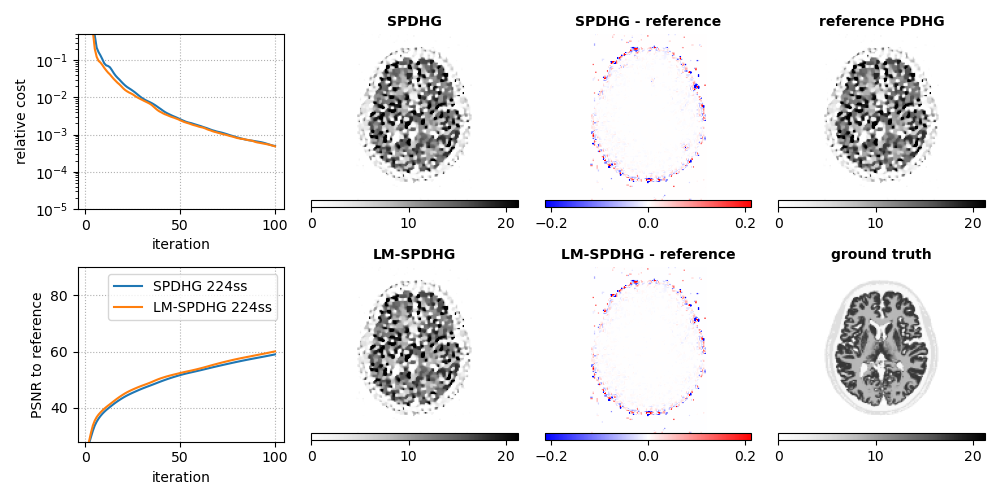
\includegraphics[width=0.9\textwidth]{./figureS1a_brain2d_counts_3.0E+05_seed_1_beta_1.0E-02_prior_TV_niter_ref_20000_fwhm_4.5_4.5_niter_100.png}
    \caption{3e5 true (5e5 prompt) counts, TV prior, $\beta = 0.01$}
  \end{subfigure}
  \vfill
  \begin{subfigure}[]{1.0\textwidth}
    \centering
    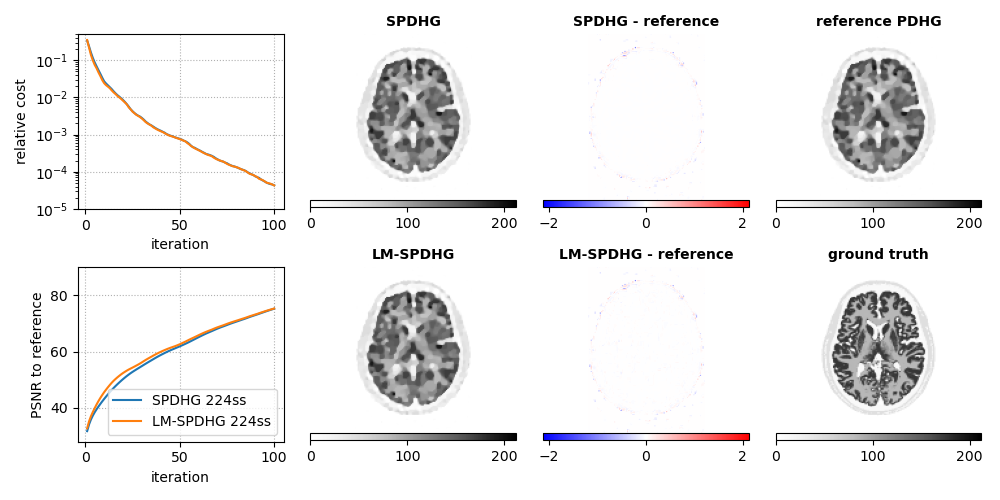
\includegraphics[width=0.9\textwidth]{./figureS1b_brain2d_counts_3.0E+06_seed_1_beta_1.0E-02_prior_TV_niter_ref_20000_fwhm_4.5_4.5_niter_100.png}
    \caption{3e6 true (5e6 prompt) counts, TV prior, $\beta = 0.01$}
  \end{subfigure}
  \caption{Same as Fig.~3 for a weaker TV prior for low (top) and high counts (bottom).}
\end{figure*}


\begin{figure*}
  \centering
  \begin{subfigure}[]{1.0\textwidth}
    \centering
    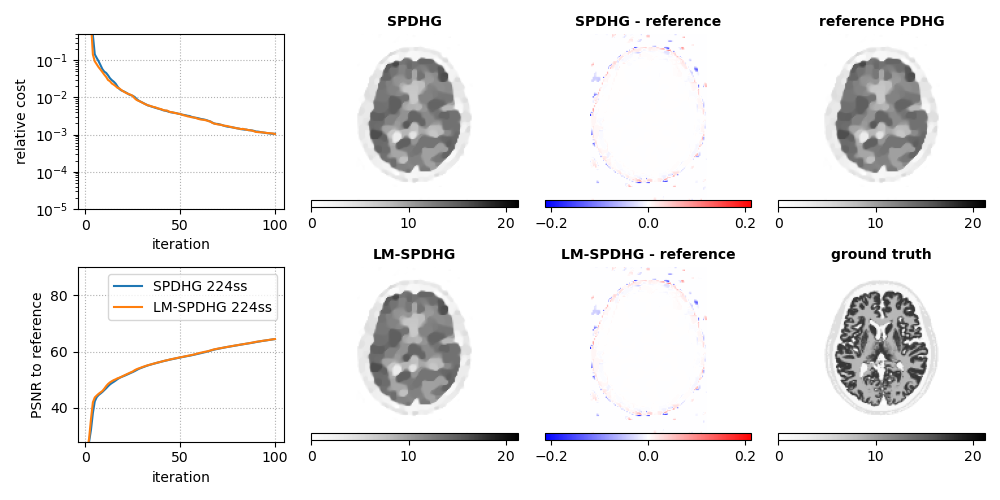
\includegraphics[width=0.9\textwidth]{./figureS2a_brain2d_counts_3.0E+05_seed_1_beta_1.0E-01_prior_TV_niter_ref_20000_fwhm_4.5_4.5_niter_100.png}
    \caption{3e5 true (5e5 prompt) counts, TV prior, $\beta = 0.1$}
  \end{subfigure}
  \vfill
  \begin{subfigure}[]{1.0\textwidth}
    \centering
    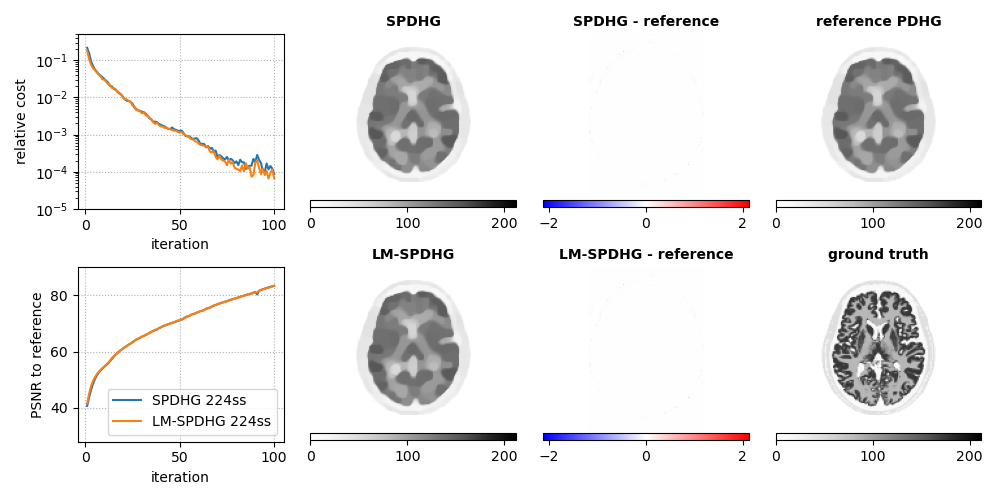
\includegraphics[width=0.9\textwidth]{./figureS2b_brain2d_counts_3.0E+06_seed_1_beta_1.0E-01_prior_TV_niter_ref_20000_fwhm_4.5_4.5_niter_100.png}
    \caption{3e6 true (5e6 prompt) counts, TV prior, $\beta = 0.1$}
  \end{subfigure}
  \caption{Same as Fig.~3 for a stronger TV prior for low (top) and high counts (bottom).}
\end{figure*}

\begin{figure*}
  \centering
  \begin{subfigure}[]{1.0\textwidth}
    \centering
    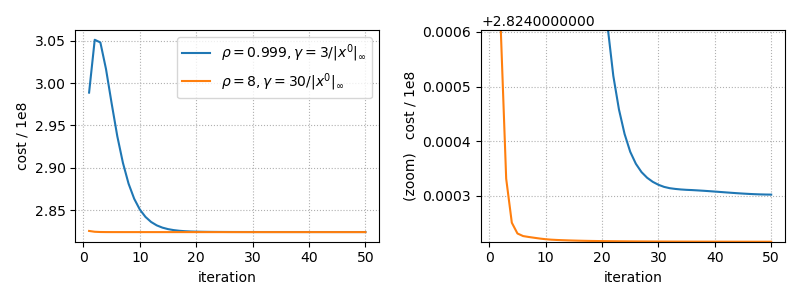
\includegraphics[width=0.6\textwidth]{./figureS3a_xcat_TV_3e-2_4e7_rho_8_conv_metrics.png}
    \caption{Evolution of the cost function for two choices of $\rho$ and $\gamma$ for the 3D
             XCAT data set.}
  \end{subfigure}
  \vfill
  \begin{subfigure}[]{1.0\textwidth}
    \centering
    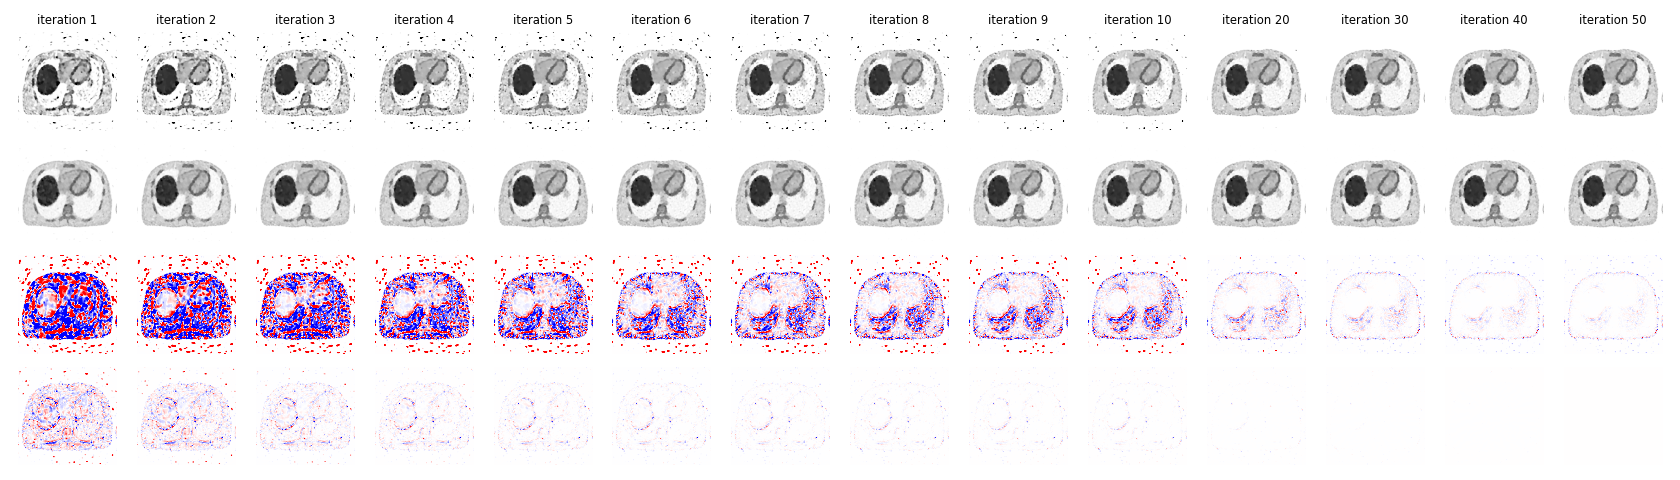
\includegraphics[width=1.0\textwidth]{./figureS3b_xcat_TV_3e-2_4e7_rho_8_conv.png}
    \caption{row 1/2: intermediate reconstructions at different iteration numbers for
                      $\rho = 0.999, \ \gamma = 3/ \| x^0 \|_\infty$ (row 1) and
                      $\rho = 8, \ \gamma = 30/ \| x^0 \|_\infty$ (row2). 
             row 3/4: absolute difference compared to the reconstruction at iteration 50
                      using ($\rho = 8, \ \gamma = 30/ \| x^0 \|_\infty$).
                      The minimum / maximum of the red-white-blue colormap is -5\% / +5\%
                      of the maximum of the reconstruction at iteration 50.}
  \end{subfigure}
  \caption{Same as Fig.~6 but including a comparison with LM-SPDHG using $\rho = 8$ and 
           $\gamma = 30 / \| x^0 \|_\infty$. 
           The latter substantially increases the speed of convergence.
           Note that increasing $\gamma$ and keeping $\rho = 0.999$ did not increase the
           speed of convergence.}
\end{figure*}


\end{document}
